\documentclass[12pt]{article}
 
\usepackage[margin=1in]{geometry} 
\usepackage{amsmath,amsthm,amssymb,amsfonts}
\usepackage{color}
\usepackage{graphicx}
\graphicspath{ {Images/} }
\usepackage{float}
\setlength{\parskip}{1em}
\usepackage{cancel}
\usepackage{longtable}
\usepackage{algorithm}
\usepackage{algpseudocode}
\usepackage{pgf,tikz,pgfplots}
\pgfplotsset{compat=1.15}
\usepackage{mathrsfs}
\usetikzlibrary{arrows}
\pagestyle{empty}
\begin{document}

\section*{Problem 3}

Given Problem 1 and 2 both dealt with only two agents computing two processes in parallel, this presents a good opportunity to move on to a problem requiring a much larger number of agents. Problem 3 revisits a problem from a previous assignment in this subject. It goes as follows, from the ELEN90026-Introduction to Optimisation: Homework 3 assignment brief verbatim.

\noindent\fbox{\begin{minipage}{39.5em}
	Consider a network with $n$ nodes and $m$ directed edges. Let $A$ be the incidence matrix of the network where its $ij$-th element is
	\begin{center}
		$A_{ij}=\begin{cases} 
		-1 & \text{Edge $j$ enters node $i$} \\
		1 & \text{Edge $j$ exits node $i$} \\
		0 & \text{otherwise.}
		\end{cases}$
	\end{center}
	Assume that two commodities flow through the network. Let $s_i$ and $t_i$ be the supply/demand of commodities 1 and 2 at node $i$, respectively. A positive value corresponds to supply and a negative value corresponds to demand. Let vectors $s\in\mathbb{R}^n$ and $t\in\mathbb{R}^n$ be obtained by stacking all $s_i$ and $t_i$, $i=1,...,n$. Let $f_i:\mathbb{R}^2\rightarrow \mathbb{R}$ be a convex function associated with the cost of transporting commodities 1 and 2 along edge $i$.
	
	The problem formulation:
	\begin{align*}
	\min_{x\in\mathbb{R},y\in\mathbb{R}}\qquad&\sum\limits_{i=1}^m f_i(x_i,y_i)\\
	s.t.\qquad &Ax=s,\quad Ay=t\\
	&x\geq 0,\quad y\geq0
	\end{align*}
\end{minipage}}\\\\

The cost function used in this problem will be $f_i(x_i+y_i)=(x_i+y_i)^2+0.1(x_i^2+y_i^2)$, for $i=1,...,m$. Let's allow the vectors $s$ and $t$ to be dense, they do not have to be sparse.

Now, the point of revisiting this problem is to apply parallel processing and observe an expected speed up in completion time versus serial processing. However, another interesting observation we can make here is to compare the completion times of solving this problem 2 core 2.90GHz Intel i7-7500U CPU versus running it on a 4 core Intel i5. But before going into that, the following describes how to obtain a solution to the optimisation problem.

In contrast to Problem 2, there are now constraint equations in the formulation, where previously Problem 2 was unconstrained. In addition, there are no shared or complicating variables in the cost function problem, it is completely separable. But the method we are going to use to solve Problem 3 will be similar to before. The dual function is
\begin{align*}
q(\alpha,\beta)&=\inf\left(\sum\limits_{i=1}^m f_i(x_i,y_i)-\alpha^\top (Ax-s)-\beta^\top(Ay-t)\right)\\
&=\alpha^\top s+\beta^\top t + \inf\left(\sum\limits_{i=1}^m f_i(x_i,y_i)-[A^\top\alpha]_ix_i-[A^\top \beta]_iy_i\right)
\end{align*}
Thus, for $i=1,...,m$, for a given $\alpha$ and $\beta$, we can let $m$ individual agents find the minimisers of $f_i(x_i,y_i)-[A^\top\alpha]_ix_i-[A^\top \beta]_iy_i$ separately, then use the subgradient to update $\alpha=\alpha-step(Ax-s)$ and $\beta=\beta-step(Ay-t)$. Note, because there are also constraints on $x,y$ being non-negative, the minimisers found by each agent must be constrained to the non-negative orthant. 


\subsection*{Convergence}

For guaranteed convergence, the graph must be connected, i.e., the incidence matrix must have rank $n-1$. Note, the chosen step size, $step$ for updating $\alpha$ and $\beta$ must decrease as $m$ increases because a larger number of columns of $A$ means more elements are being summed up when doing $Ax$ and $Ay$.

\begin{figure}[H]
	\centering
	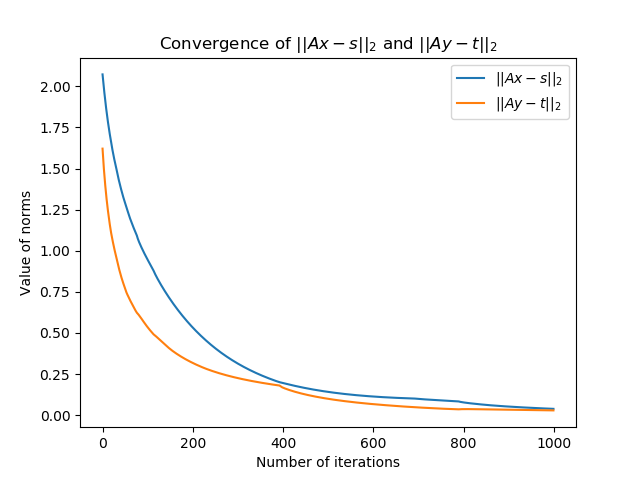
\includegraphics[scale=0.91]{Problem3-Convergence.png}
	\caption{A problem with a scale-free graph with 20 nodes.}
\end{figure}

\subsection*{Computational Overhead}

For this problem, we are trying to simulate $m$ agents each computing 1 processes in parallel. This is not possible with the i7 dual-core CPU that can run at most 4 processes in parallel. The best that can be done is to use the Pool object in Python's multiprocessing module and the method Pool.map. The $m$ processes are put into a pool, then offloaded to workers, which will iterate through all the tasks in the pool and compute them in parallel. With 4 logical processors, we have a maximum of 4 workers, so only 4 processes can be carried out in parallel. The following plot compares the completion time of parallelising with the Pool object versus solving the problem in series.

\begin{figure}[H]
	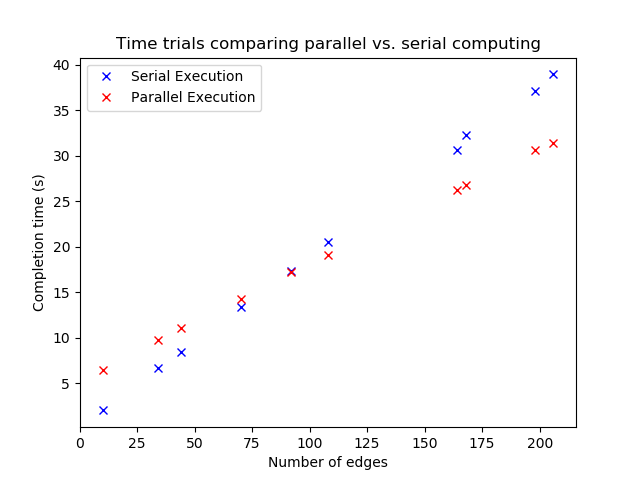
\includegraphics[scale=1]{Problem3-TimeTrial.png}
	\caption{Run on 2.90GHz Intel i7-7500U CPU with 2 cores (4 logical processors).}
\end{figure}

As expected, for a small problem size, the overhead of spawning processes in parallel means that parallel processing does worse than serial processing in terms of completion times. However, solving the problem by computing processes in parallel becomes faster than serial computing when the problem size increases. But we've seen this in Problem 1 and 2 already. It is more interesting to oberve the same code run on a different machine.

\begin{figure}[H]
	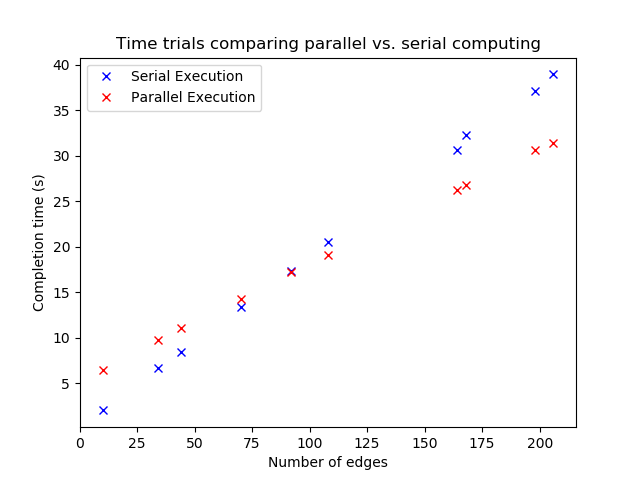
\includegraphics[scale=1]{Problem3-TimeTrial.png}
	\caption{Run on 2.90GHz Intel i7-7500U CPU with 2 cores (4 logical processors).}
\end{figure}

\subsection*{How to Run}

\subsubsection*{The above examples}

Make sure you are in the correct directory. Then to run the test that generated the above plots, execute the \textbf{main.py} file, i.e. use the command

\noindent \textbf{$>>>$python main.py}

\subsubsection*{Function Descriptions}

The function \textbf{parallel.do\_parallel}, description.

Syntax: do\_parallel(max\_iter,step\_size,incidence\_matrix,s,t,verbose=False)

Parameter values:
\begin{itemize}
	\item max\_iter, Required. Number of iterations for the subgradient method.
	\item alpha, Required. Step size for the subgradient method.
	\item incidence\_matrix, Required. The incidence matrix of a connected graph as described above.
	\item s, Required. Vector of supply/demand of commodity 1 of every node. Elements of s must sum to 0.
	\item t, Required. Vector of supply/demand of commodity 2 of every node. Elements of t must sum to 0.
	\item verbose, Default False. Print results to screen.
\end{itemize}

Outputs:
\begin{itemize}
	\item Output 1. List containing $||Ax-s||_2$ for all iterations of the subgradient method.
	\item Output 2. List containing $||Ay-t||_2$ for all iterations of the subgradient method.
	\item Output 3. Completion time.
\end{itemize}

\end{document}